\documentclass[letterpaper,
               keeplastbox,
               %boxit,
               %titlepage,   % separate title page
               %refpage      % separate references
               nospread,
               biblatex,
              ]{jacow}
%
% CHANGE SEQUENCE OF GRAPHICS EXTENSION TO BE EMBEDDED
% ----------------------------------------------------
% test for XeTeX where the sequence is by default eps-> pdf, jpg, png, pdf, ...
%    and the JACoW template provides JACpic2v3.eps and JACpic2v3.jpg which
%    might generates errors, therefore PNG and JPG first
%
\makeatletter%
	\ifboolexpr{bool{xetex}}
	 {\renewcommand{\Gin@extensions}{.pdf,%
	                    .png,.jpg,.bmp,.pict,.tif,.psd,.mac,.sga,.tga,.gif,%
	                    .eps,.ps,%
	                    }}{}
\makeatother

% CHECK FOR XeTeX/LuaTeX BEFORE DEFINING AN INPUT ENCODING
% --------------------------------------------------------
%   utf8  is default for XeTeX/LuaTeX 
%   utf8  in LaTeX only realises a small portion of codes
%
\ifboolexpr{bool{xetex} or bool{luatex}} % test for XeTeX/LuaTeX
 {}                                      % input encoding is utf8 by default
 {\usepackage[utf8]{inputenc}}           % switch to utf8

\usepackage[USenglish]{babel}

\usepackage[final]{pdfpages}
\usepackage{multirow}
\usepackage{ragged2e}

% Packages to comment out before final release:
\usepackage{todonotes}
\presetkeys{todonotes}{inline}{}
% END packages to comment out before final release
\usepackage{subcaption}
%
% if BibLaTeX is used
%
\ifboolexpr{bool{jacowbiblatex}}%
 {%
  \addbibresource{napac2022.bib}
 }{}
\listfiles


%
% command for typesetting a \section like word
%
\newcommand\SEC[1]{\textbf{\uppercase{#1}}}

%%
%%   Lengths for the spaces in the title
%%   \setlength\titleblockstartskip{..}  %before title, default 3pt
%%   \setlength\titleblockmiddleskip{..} %between title + author, default 1em
%%   \setlength\titleblockendskip{..}    %afterauthor, default 1em

%\copyrightspace %default 1cm. arbitrary size with e.g. \copyrightspace[2cm]

% testing to fill the copyright space
%\usepackage{eso-pic}
%\AddToShipoutPictureFG*{\AtTextLowerLeft{\textcolor{red}{COPYRIGHTSPACE}}}

\begin{document}

\title{Measurements of the five-dimensional phase space distribution of an intense ion beam}

\author{A. Hoover\thanks{hooveram@ornl.gov}, K. Ruisard, A. Alexandrov, A. Zhukov, S. Cousineau, ORNL, Oak Ridge, Tennessee, USA}
	
\maketitle

%
\begin{abstract}
No simulation of intense beam transport has accurately reproduced measurements at the level of beam halo. One potential explanation of this discrepancy is a lack of knowledge of the initial distribution of particles in six-dimensional (6D) phase space. A direct 6D measurement of an ion beam was recently performed at the Spallation Neutron Source (SNS) Beam Test Facility (BTF), revealing nonlinear transverse-longitudinal correlations in the beam core that affect downstream evolution. Unfortunately, direct 6D measurements are limited in resolution and dynamic range; here, we discuss the use of three slits and one screen to measure a 5D projection of the 6D phase space distribution, overcoming these limitations at the cost of one dimension. We examine the measured 5D distribution before and after transport through the BTF and compare to particle-in-cell simulations. We also discuss the possibility of reconstructing the 6D distribution from 5D and 4D projections.
\end{abstract}

\section{Introduction}


The performance of high-intensity particle accelerators is limited by beam halo formation — the emergence of a low-density region of phase space far from the beam core. Halo suppression will become necessary in future accelerators with fractional beam loss requirements of $10^{-6}$ or below. Accurate measurement and prediction of beam halo is needed for this task.

Previous attempts to benchmark simulations with measurements at the halo level — a density at or below 10$^{-4}$ relative to the beam core — have been unsuccessful \cite{LEDA, Groening}. It is possible that (i) the physics encoded in the simulation model are inaccurate/incomplete, (ii) the lattice model is inaccurate/incomplete, (iii) the initial bunch particles are inaccurately distributed in phase space. 

The Spallation Neutron Source (SNS) Beam Test Facility (BTF) is poised to address (ii) and (iii). The BTF is a replica of the front-end of the SNS linac — the H$^-$ ion source, low-energy beam transport (LEBT), radio-frequency quadrupole (RFQ) and medium energy beam transport (MEBT) — followed by a 180-degree bend and a twenty-cell FODO transport line. There are two emittance measurement stations: one just after the RFQ and one after the FODO line. The two-dimensional (2D) horizontal/vertical phase space distribution can be measured at either station with a dynamic range above $10^6$. The 6D phase space distribution can be measured at the first station.

Measurements of the 6D phase space distribution are currently limited in dynamic range ($10^1$) and resolution (10 points per dimension). Improvements to the scan efficiency are in development. In this paper, we discuss the use of three slits and one screen to measure a 5D projection of the 6D phase space distribution, overcoming these limitations at the cost of one dimension. 

\section{Efficient 5D phase space measurement}

The measurement apparatus shown in Fig.~\ref{fig:1} consists of two vertical slits to select the horizontal position $x$ and momentum $x'$, a vertical slit to select the vertical position $y$, and a scintillating screen after a dipole bend. The vertical momentum $y'$ is linearly related to the vertical position on the screen; the energy deviation $w$ is a function of the horizontal position on the screen as well as the $x$ and $x'$ selected by the upstream slits. The scan consists of a series of "sweeps" where the vertical slits are held fixed while the horizontal slit moves at a fixed speed, collecting the image on the screen on every beam pulse. A rectilinear scan pattern is employed with a linear correlation between $x$ and $x'$ to align the grid with the $x$-$x'$ distribution.

[The dynamic range of the measurements is estimated from the camera integral during the scan, shown in Fig.~\ref{fig:}.]

Slit-scan phase space measurements produce a collection of points in space and a scalar value associated with each point. This data must be linearly interpolated on a regular grid. The scan pattern becomes highly relevant at this point: linear interpolation is infeasible in high-dimensional spaces for even a small number of points due to the poor scaling of Delaunay triangulation \cite{}. In our case, the data can be interpolated as follows. First, for each $x$, $x'$, and $y$, the horizontal image coordinate $x_3$ is converted to phase space coordinate $w(x_3, x, x', M)$, where $M$ is the linear transfer matrix from the first slit to the screen, and the image is interpolated along its horizontal axis onto a regular $w$ grid. Second, the vertical image coordinate $y_3$ is converted to phase space coordinate $y'(y, y_3, M)$ and the image is interpolated along its vertical axis onto a regular $y'$ grid. Third, for each $x$ and $x'$, the 3D $y$-$y'$-$w$ image is interpolated along the $y$ axis, which is irregularly spaced due to the acceleration of the slit at its turning points. Third, the $x$-$x'$ distribution is interpolated onto a regular $x$-$x'$ grid for each pixel in the 3D image. This final step can be broken into two 1D interpolations if the scan progresses along vertical or horizontal lines in $x$-$x'$ space, as is the standard practice in current BTF measurements.




\section{Measurements of the initial distribution in the BTF}

We begin by examining the measured 5D distribution at the first emittance station, just after the RFQ. The beam current during the measurement was stable at [] mA. [] points were collected over [] hours as the slits traversed a ? x ? x ? grid. The camera integral during the scan is shown in Fig.~\ref{fig:}. Fig.~\ref{fig:VS06_corner} shows the 2D projections of the measured 5D phase space distribution in a logarithmic color scale. The density profiles vary smoothly in all projections and there are apparently no correlations between the planes. 
%
\begin{figure}[!b]
    \centering
    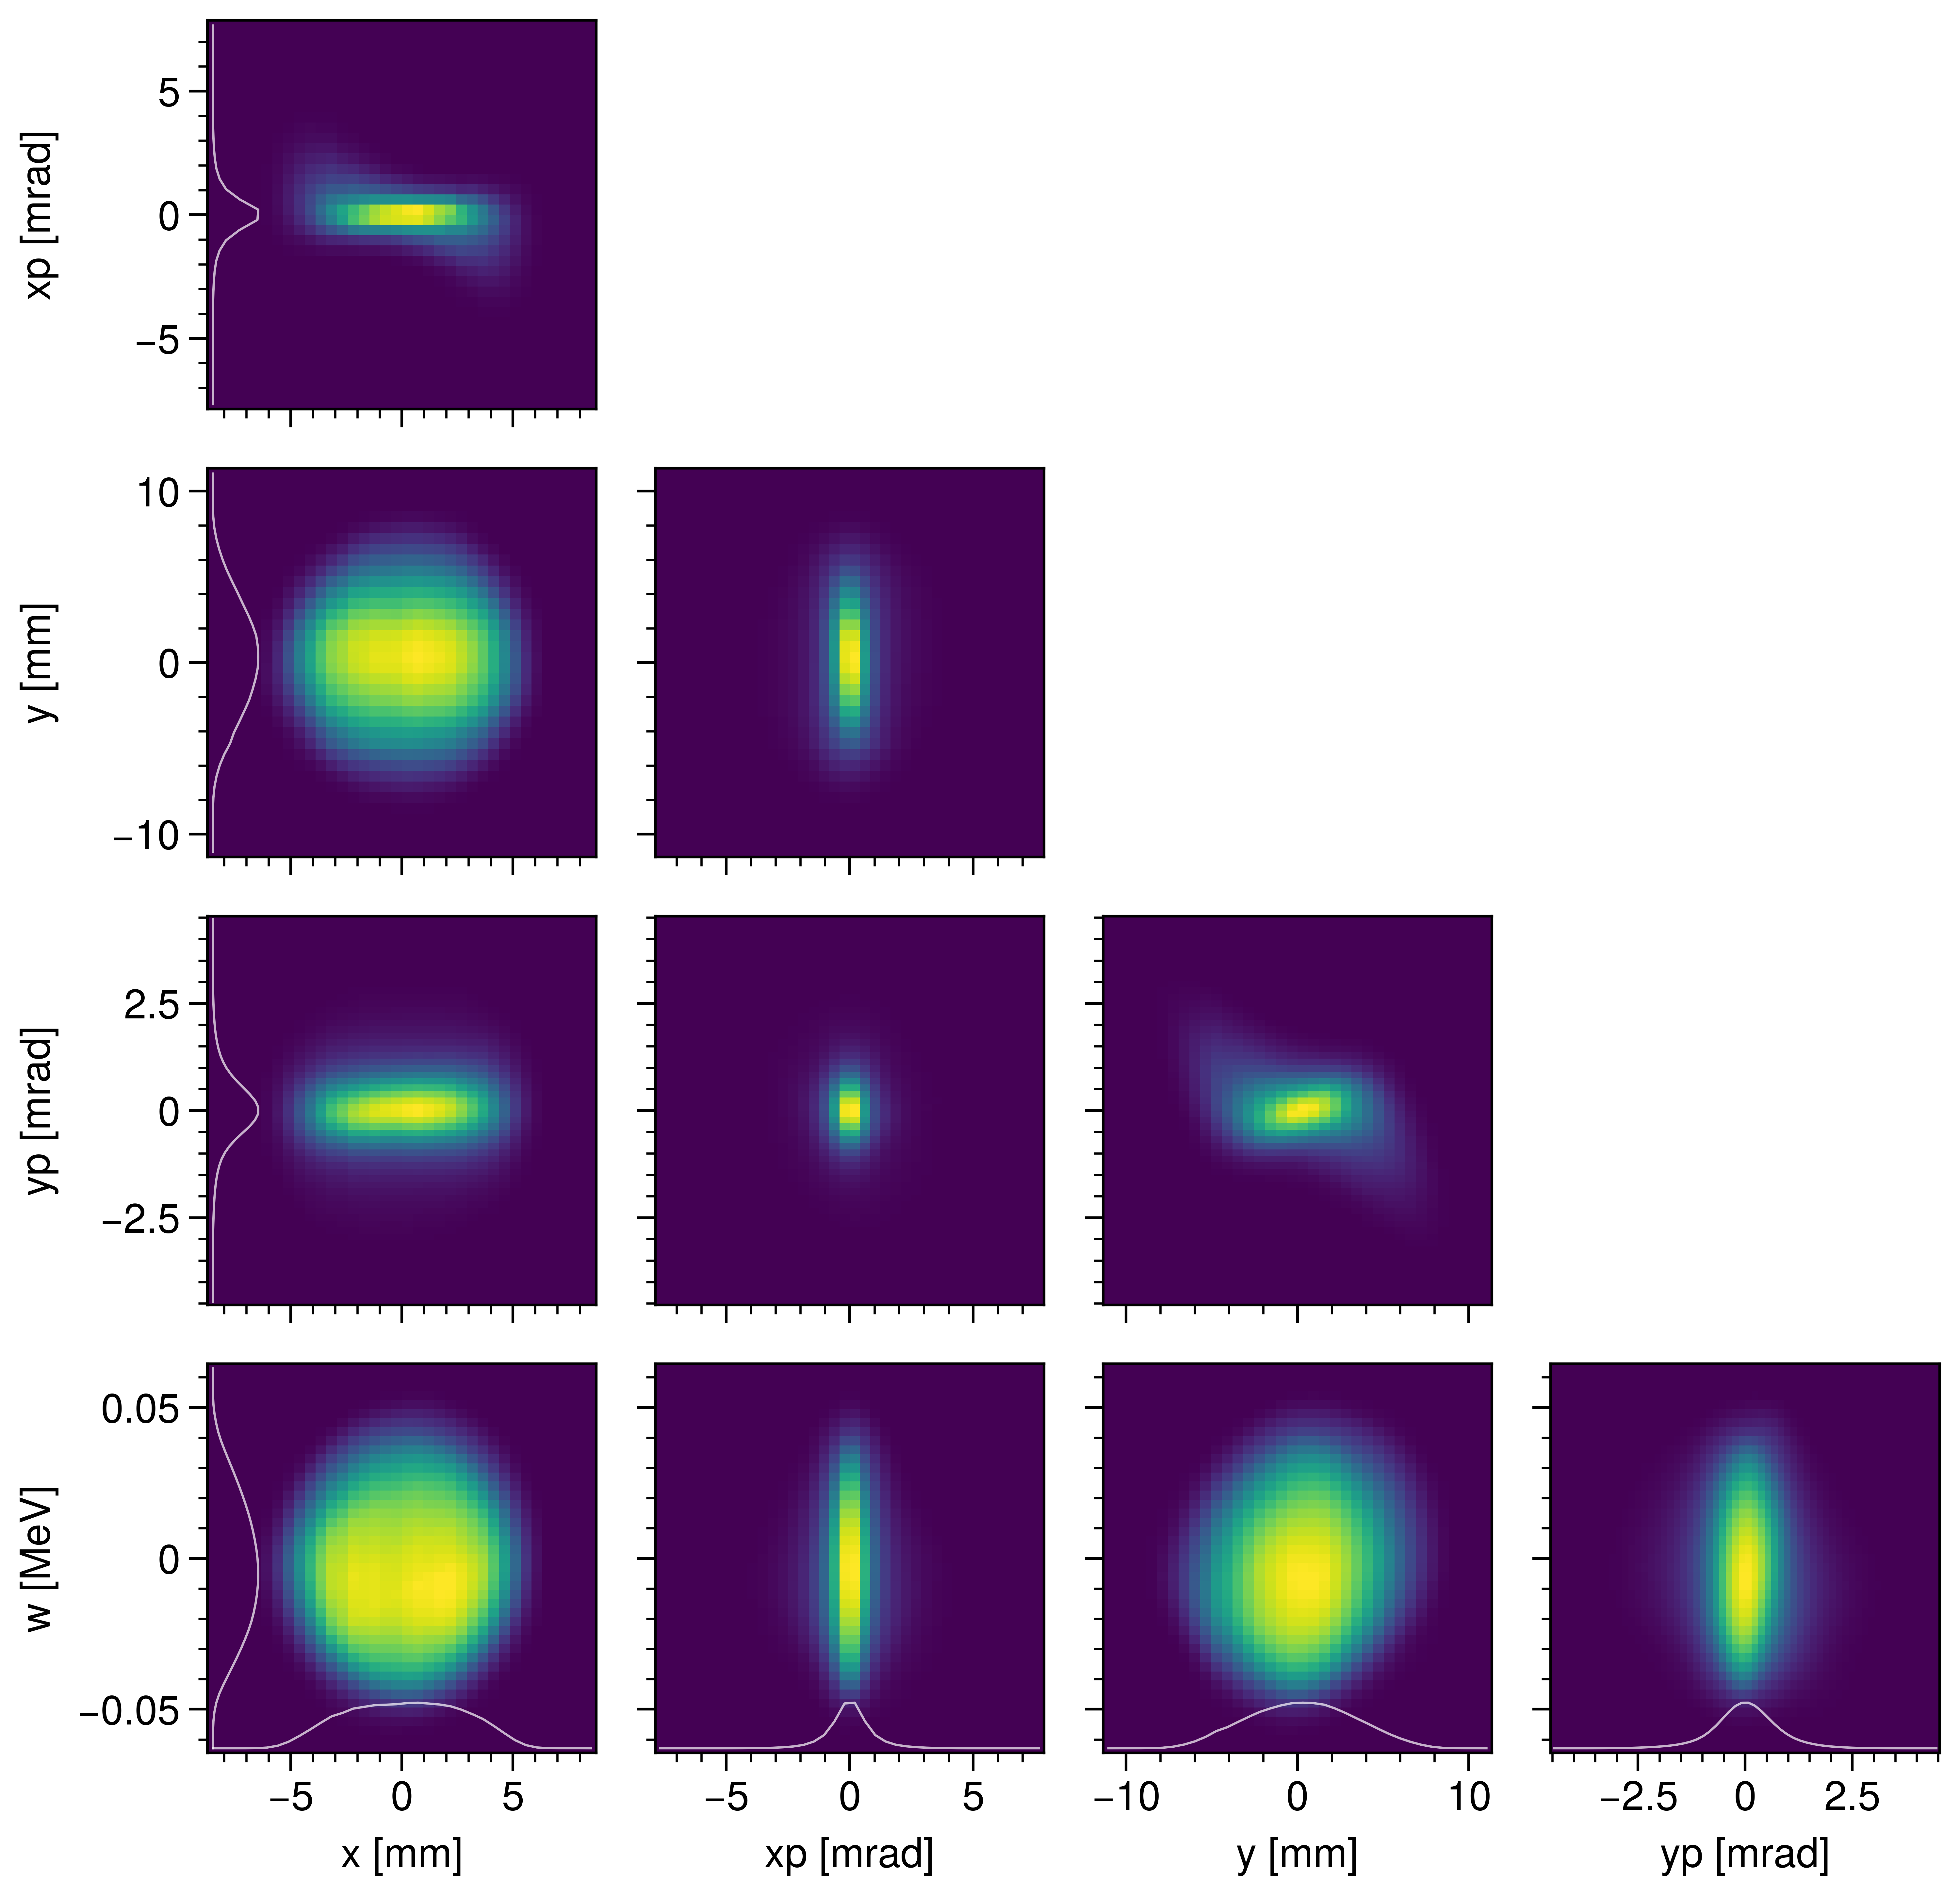
\includegraphics[width=\columnwidth]{VS06_corner.png}
    \caption{1D and 2D projections of the measured 5D phase space distribution at the first emittance station in the BTF.}
    \label{fig:VS06_corner}
\end{figure}
%

Previous beam shape monitor (BSM) measurements of the beam exiting the RFQ have revealed nonlinear transverse-longitudinal correlations in the beam core: the energy distribution of particles at the center of transverse phase space ($x \approx x' \approx y \approx y' \approx 0$) is hollow and bimodal while the full projection is unimodal (see Fig.~\ref{fig:hollow_a}). This is a space-charge-driven effect \cite{Ruisard2021-hollow} and has a clear dependence on the beam intensity (see Appendix \ref{app:A}). 

The relationship between the energy and transverse coordinates has been examined using partial projections of the  distribution \cite{CatheyPRL, Ruisard2021-hollow}; i.e., by inserting multiple slits upstream of the BSM. Such projections make clear the multi-dimensional nature of the correlation and are repeated for our 5D measurement in Fig.~\ref{fig:hollow}.

%
\begin{figure}[!t]
    \centering
    \begin{subfigure}{\columnwidth}
        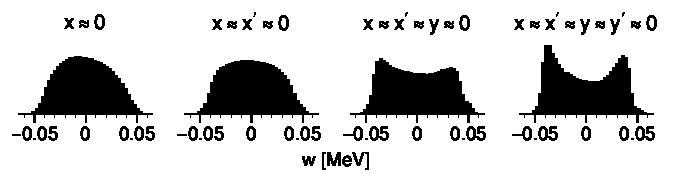
\includegraphics[width=\textwidth]{w_slices.pdf}
        \caption{}
        \label{fig:hollow_a}
    \end{subfigure}
    \begin{subfigure}{\columnwidth}
        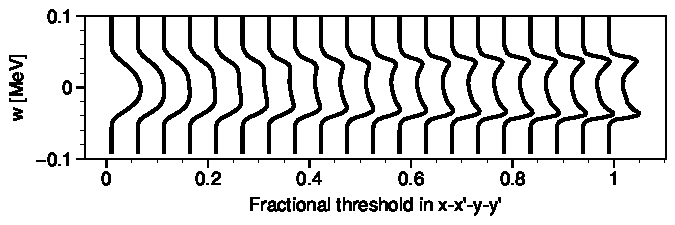
\includegraphics[width=\textwidth]{4Dcontour_dE2.pdf}
        \caption{}
        \label{fig:hollow_b}
    \end{subfigure}
    \caption{Hollow energy distribution in the beam core measured at the first emittance station in the BTF. (a) Energy projection of the 5D phase space distribution as it is sliced in transverse phase space. (b) Each curve is the energy distribution of particles within a density contour in transverse phase space.}
    \label{fig:hollow}
\end{figure}
%

The 5D measurement provides a more complete picture: it reveals the extent of the hollow energy core in the transverse phase space. For example, Fig.~\ref{fig:contour_slices_a} plots the energy distribution within a shrinking volume in 4D phase space. For each threshold $t$, we integrate the 5D array along the $w$ axis and locate all elements whose value is less than $t$ times the maximum element in the 4D array. We then mask these indices in the 5D array before projecting it onto the $w$ axis. A hollow energy distribution begins to emerge at the $10^{-1}$ contour in 4D phase space.

The effect of this feature on the long-term  beam dynamics is not yet known due to the lack of a realistic 6D simulation bunch. Some insight was gained in \cite{Ruisard2021-IPAC} by propagating a beam through the RFQ in simulation, then through the SNS linac before and after removing all inter-plane correlations from the distribution. (Although beams generated by RFQ simulations are significantly different than measurements in a root-mean-square sense, they exhibit hidden correlations in 6D phase space that are qualitatively similar to measurements.) Perhaps surprisingly, the two cases developed significant differences even in the root-mean-square beam sizes. 



\section{5D simulation benchmark}

While the 6D measurement can only be performed at the first emittance station, the 5D measurement can be performed at either emittance station. This provides a unique opportunity for a 5D simulation benchmark. In the next section, we will discuss the possibility of generating a 6D simulation bunch from the 5D measurement — for now, we generate initial bunches by independently sampling from 2D measurements such that $f(x,x',y,y',z,z') = f(x,x')f(y,y')f(z,z')$. 

Fig.~\ref{fig:VS34} compares the measured 5D phase space distribution at the second emittance station to a simulation. The scan traversed a $64 \times 64 \times 64$ grid, collecting ? images in ? hours. The simulation was performed with a 3D fast Fourier transform space charge solver on a ?x?x? mesh with one million macro-particles.
%
\begin{figure*}[!t]
    \centering
    \begin{subfigure}{0.48\textwidth}
        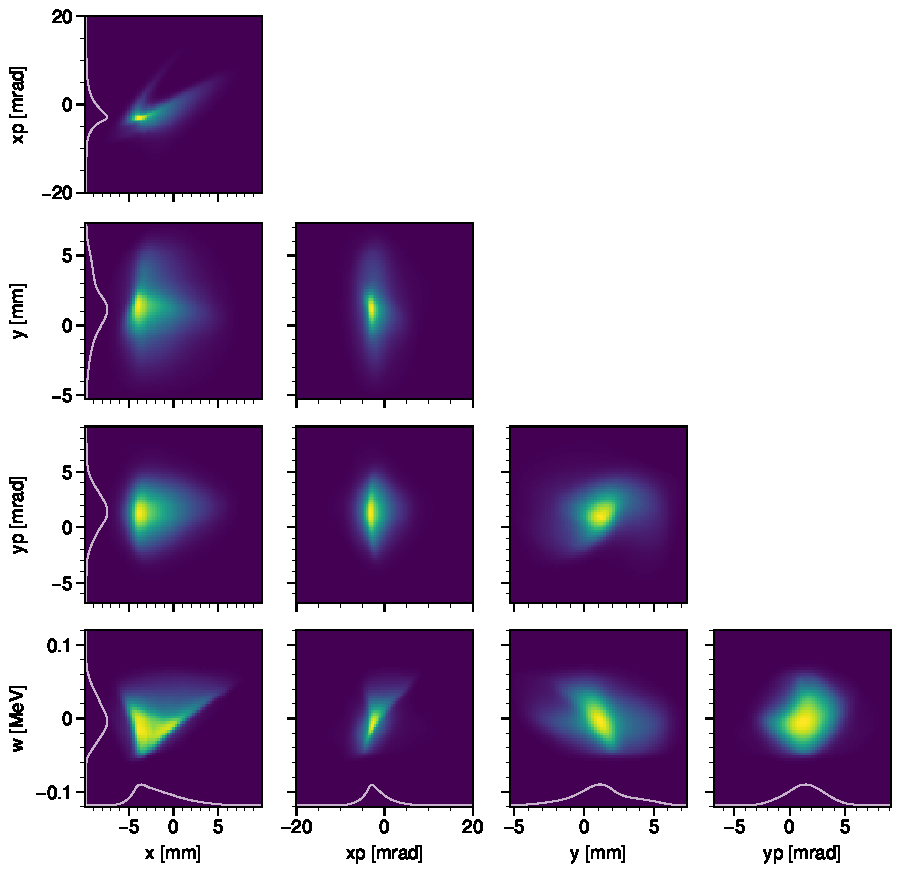
\includegraphics[width=\textwidth]{VS34_corner.pdf}
        \caption{}
        \label{fig:VS34_a}
    \end{subfigure}
    \hfill
    \hspace{0.1cm}
    \hfill
    \begin{subfigure}{0.48\textwidth}
        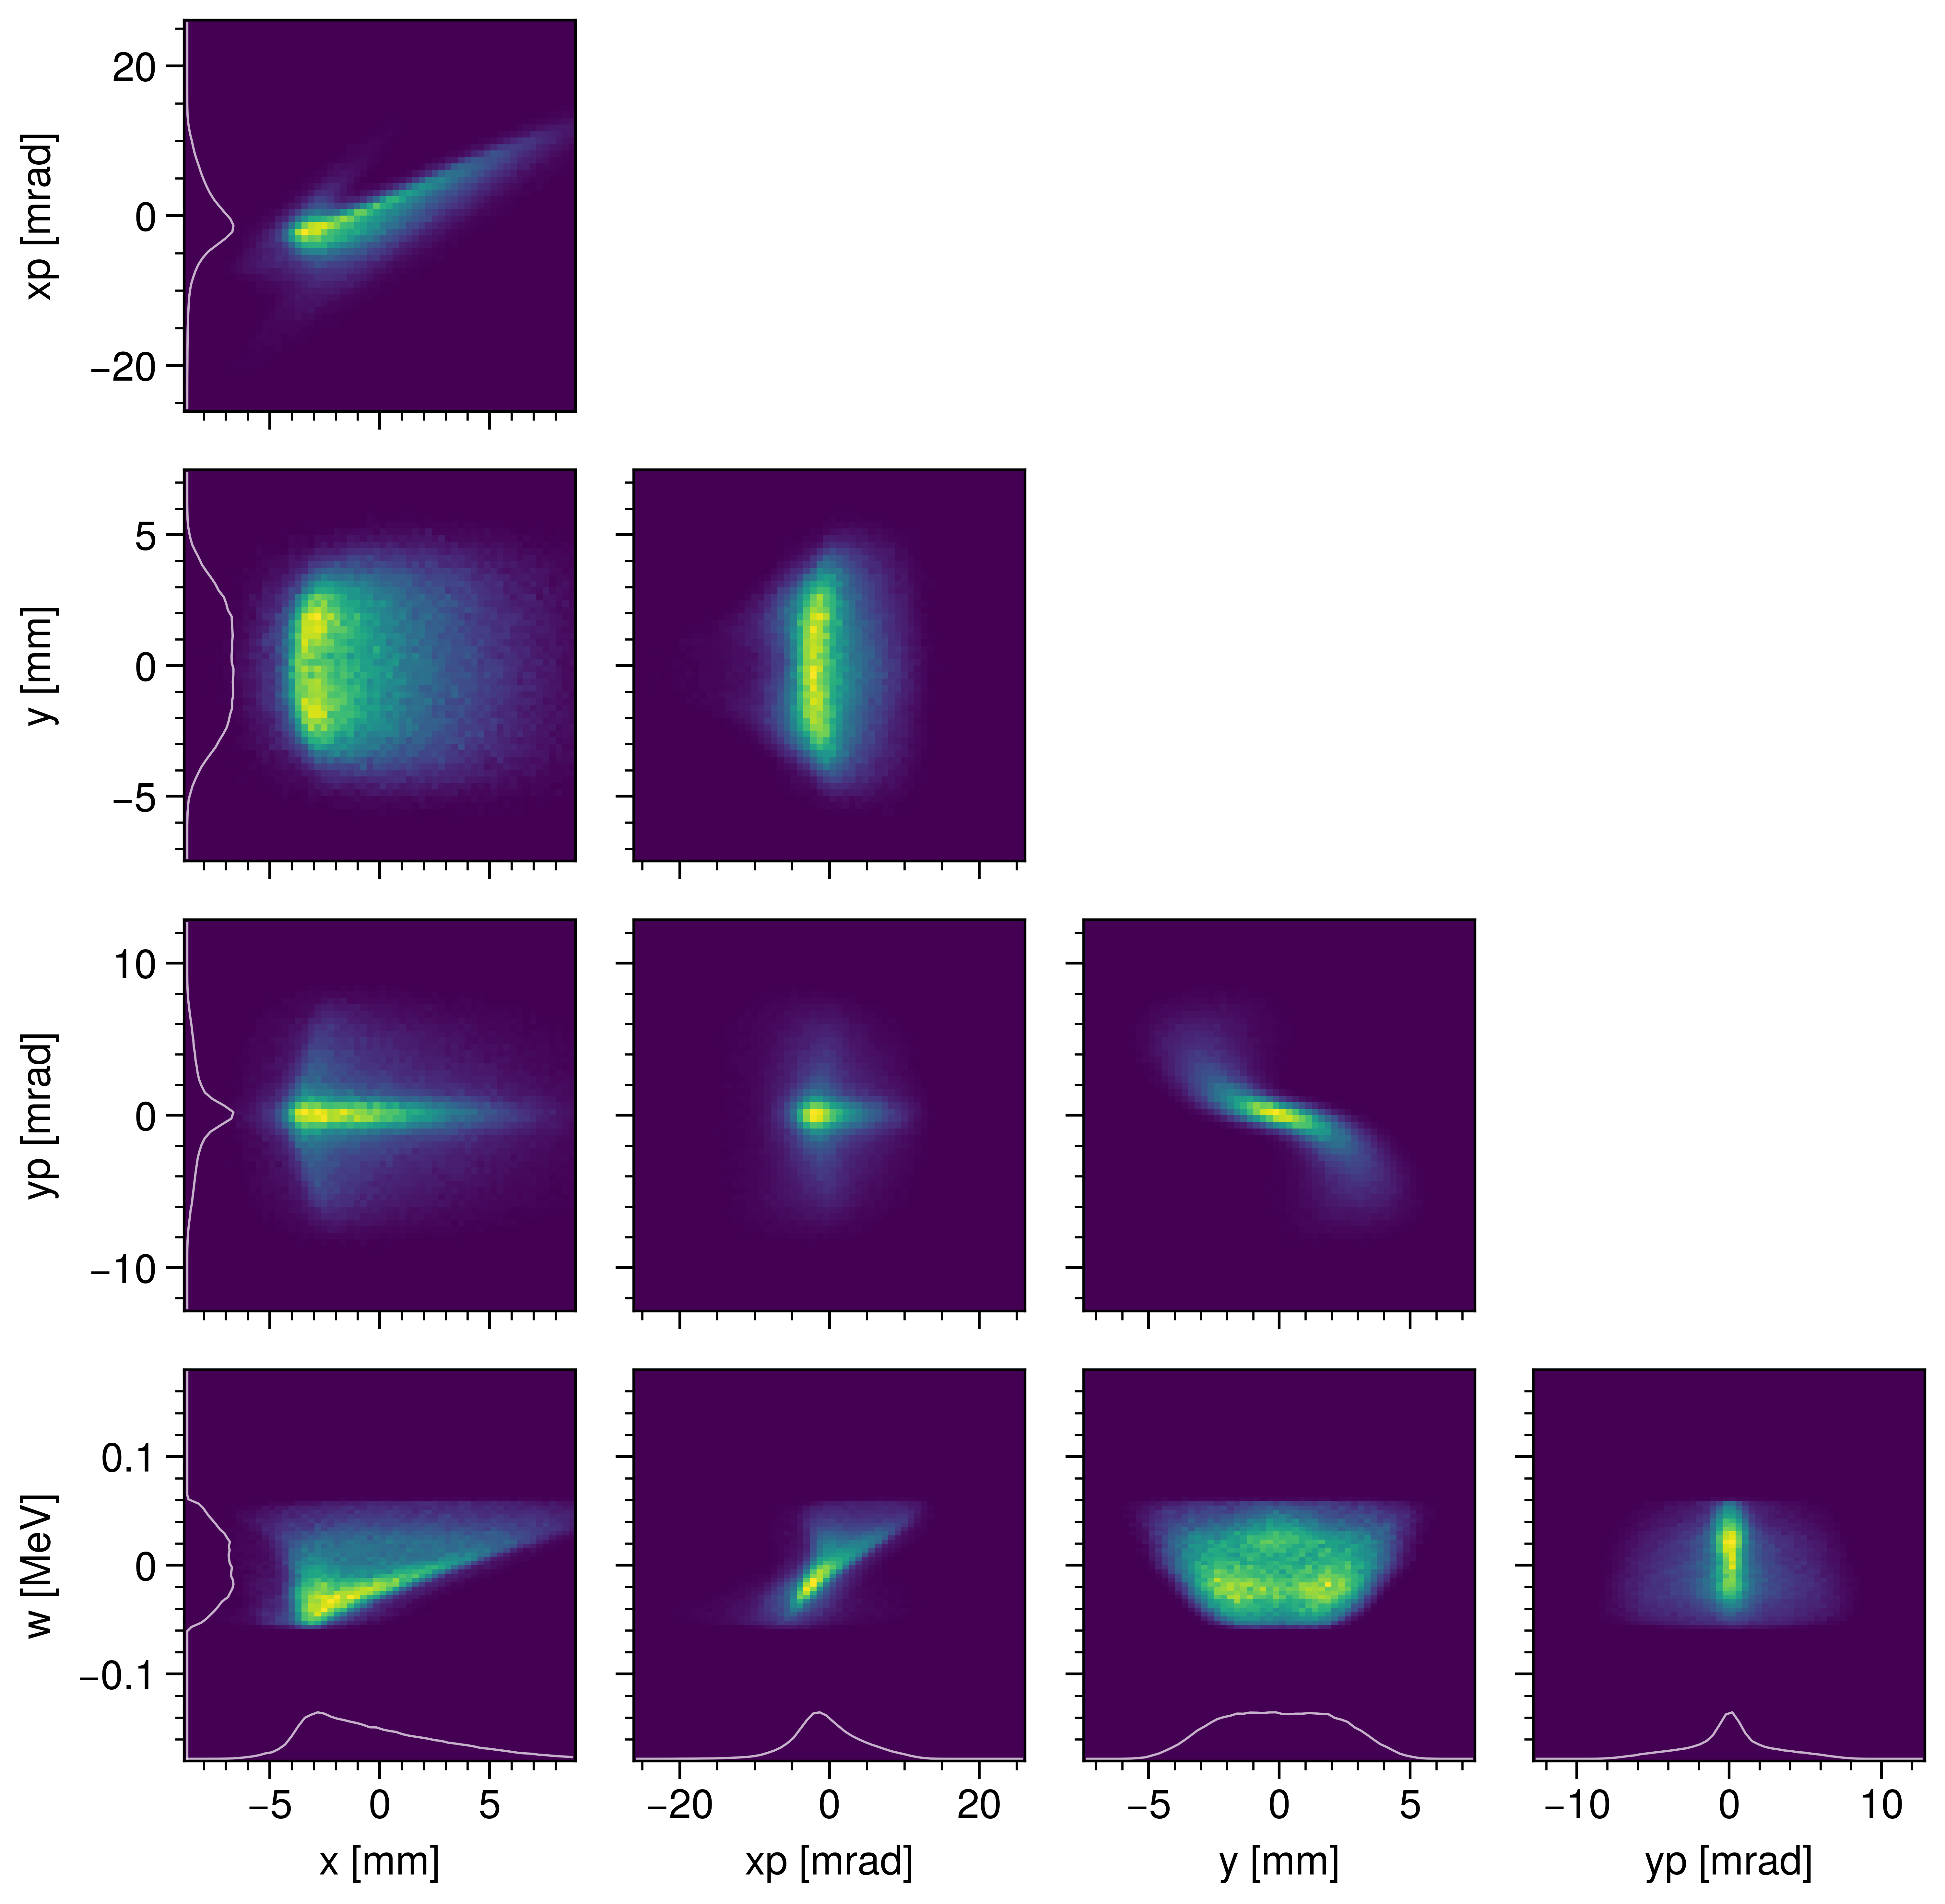
\includegraphics[width=\textwidth]{VS34_corner_sim.png}
        \caption{}
        \label{fig:VS34_b}
    \end{subfigure}
    \vfill
    \vspace*{0.2cm}
    \vfill
    \begin{subfigure}{\textwidth}
        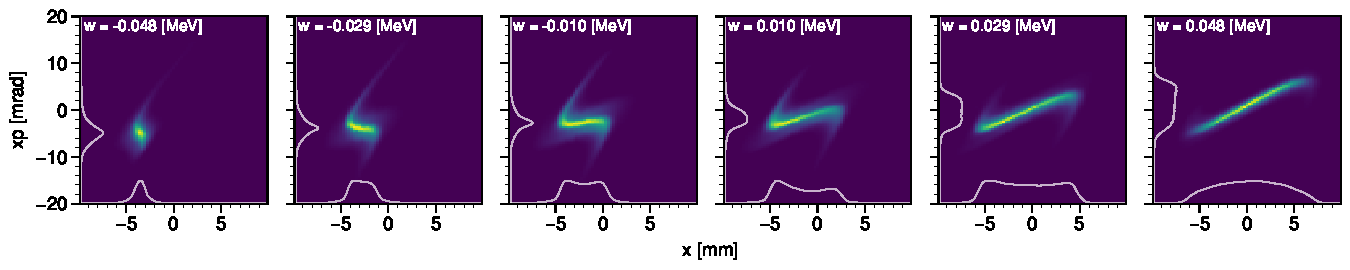
\includegraphics[width=\textwidth]{VS34_energy_slice.pdf}
        \caption{}
        \label{fig:VS34_c}
    \end{subfigure}
    \vfill
    \vspace*{0.2cm}
    \vfill
    \begin{subfigure}{\textwidth}
        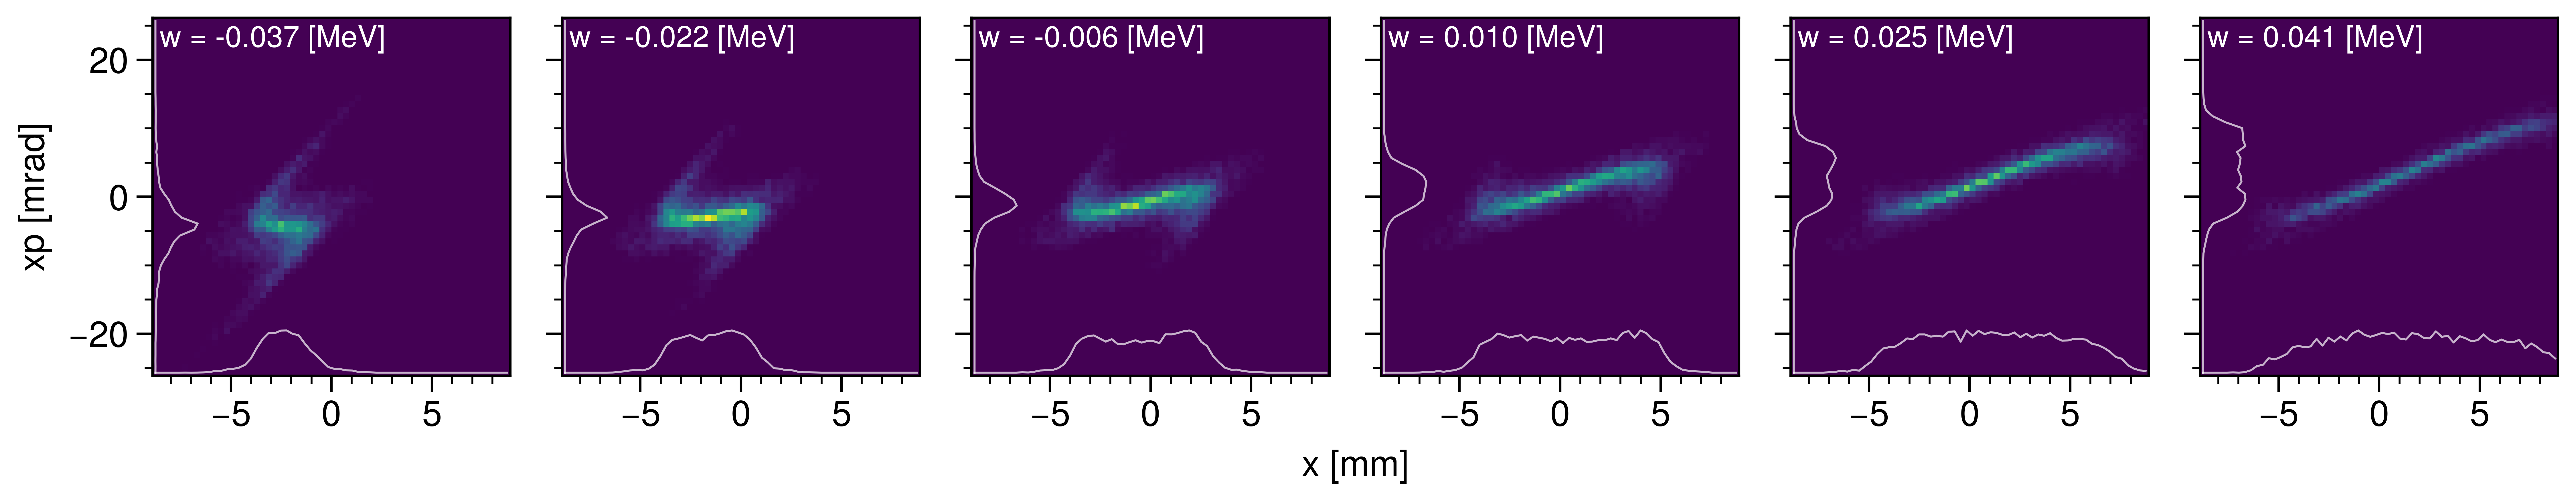
\includegraphics[width=\textwidth]{VS34_energy_slice_sim.png}
        \caption{}
        \label{fig:VS34_d}
    \end{subfigure}
    \caption{Comparison between the measured and simulated 5D phase space distribution at the second emittance station. (a) Measured 1D/2D projections. (b) Simulated 1D/2D projections. (c) Measured $x$-$x'$ distribution for different energy slices. (d) Simulated $x$-$x'$ distribution for different energy slices. The initial bunch in the simulation was generated by independently sampling measured 2D phase spaces distributions at the first emittance station.}
    \label{fig:VS34}
\end{figure*}
%

The reasonable agreement in $x$-$x'$-$w$ space — especially clear in the slice-emittances in Fig.~\ref{fig:VS34_c} and Fig.~\ref{fig:VS34_d} — was expected from previous successful benchmarks of the $x$-$x'$ distribution in \cite{Ruisard2021-IPAC}. The disagreement in the vertical plane is unresolved but may be due to vertical dispersion combined with unidentified quadrupole misalignment or offset of the beam centroid.


\section{Reconstructing the 6D distribution from 5D and 4D projections} 

Perhaps the 6D distribution can be recovered from lower-dimensional projections. Doing so would allow realistic simulation bunches to be generated from high-resolution and relatively high-dynamic-range measurements, which is not currently possible with direct 6D measurements. Letting $z$ and $z'$ be the longitudinal phase space coordinates, the 5D projection $f(x, x', y, y', z')$ can be measured using the method described in this paper, while the 4D projection $f(x, x', z, z'$ can be measured using two vertical slits and a BSM \cite{Ruisard2021-long}. The problem is then to reconstruct $f(x, x', y, y', z, z')$ consistent with the measured $f(x, x', y, y', z')$ and $f(x, x', z, z')$. 

We propose several approaches here. A naive solution would be $f(x, x', y, y', z, z') = f(x, x', y, y', z') f(z)$; however, this assumes no correlation between $z$ and $z'$, which are strongly correlated in reality. A simple but promising solution is the first generate a 5D particle distribution, then add the $z$-$z'$ correlation ``by hand", assuming $z' a\approx z + \Delta$ where $a$ is a constant and $\Delta$ is a small random variable. This will be our first attempt.

More interesting is the case of an arbitrary $z$ distribution. An almost identical problem has been encountered in astrophysics: the Gaia satellite has measured the phase space coordinates of many stars in the Milky Way galaxy, but a large fraction of the measurements contain only five of the six coordinates. Bayesian neural networks have been employed to predict the missing coordinate. 

Another approach is to treat the problem as a tomographic image reconstruction. For example, the iterative Maximum Entropy (MENT) algorithm could be used, which selects the maximum entropy image among those consistent with the measured projections. It is unknown if MENT (or other image reconstruction algorithms) can easily scale from two to six dimensions.


\section{Conclusion}

Bla bla

\section{Appendix}\label{app:A}


\printbibliography

\end{document}